\documentclass[letterpaper, reqno,11pt]{article}
\usepackage[margin=1.0in]{geometry}
\usepackage{color,latexsym,amsmath,amssymb,graphicx,float,listings,tikz}
\usepackage{hyperref}

\hypersetup{
colorlinks=true,
linkcolor=magenta,
filecolor=magenta,
urlcolor=cyan,
}

\lstset{
  basicstyle=\ttfamily,
  columns=fullflexible,
  frame=single,
  breaklines=true,
  postbreak=\mbox{\textcolor{red}{$\hookrightarrow$}\space},
}

\graphicspath{ {images/} }

\begin{document}
\pagenumbering{arabic}
\title{Math 406 Homework 5}
\date{17/11/23}
\author{Xander Naumenko}
\maketitle

{\medskip\noindent\bf Question 1a.} For all functions $v$ in some class, the following must be true:
\[
\int_{0}^{1}v(u''+k^2u-f)dx=0
.\]
Integrating by parts:
\[
\int_0^{1}-u'v'+k^2uv-fvdx+v(1)\beta-v(0)u'(0)=0\implies \int_0^{1}u'v'dx=k^2\int_0^{1}uvdx-\int_0^{1}fvdx+\beta v(1)
.\]
Thus the weak form is to find $u\in H_\alpha^{1}$ such that $\int_0^{1}u'v'dx=k^2\int_0^{1}uvdx-\int_0^{1}fvdx+\beta v(1)\forall v\in H_0^{1}$.

{\medskip\noindent\bf Question 1b.} Since we used the strong form to derive the weak form while relaxing constraints, the strong form always implies the weak form. For the other direction:
\[
\int_{0}^{1}u'v'dx=k^2\int_0^{1}uvdx-\int_0^{1}fvdx+\beta v(1)\forall v
.\]
Assuming sufficient differentiability, we can go backwards using integration by parts:
\[
\implies u'v\bigg|_0^{1}-\int_0^{1}v\left( u''+k^2u-f \right) dx-\beta v(1)=0=v(1)\left( u'(1)-\beta \right) -\int_0^{1}v\left( u''+k^2u-f \right) dx
.\]
Since this holds for all $v$, we have $u''+k^2u=f$, $u'(1)=\beta$ and $u(0)=\alpha$ (since $u\in H_\alpha^{1}$) as required.

{\medskip\noindent\bf Question 1c.} Let $u^{h}(x)=\sum_{n=0}^{N}u_nN_n(x)$, where $N_n(x)$ are the basis functions. Similarly let $v^{h}(x)=\sum_{n=1}^{N}v_nN_n(x)$. Using the weak form derived above, we need to find $u^{h}\in V_\alpha^{h}$ such that:
\[
\int_0^{1}\left(\alpha N_0'+\sum_{n=1}^{N}u_nN_n'\right)\left( \sum_{m=1}^{N}v_mN_m' \right) dx=k^2\int_0^{1}\left( \alpha N_0+\sum_{n=1}^{N}u_nN_n \right) \left( \sum_{m=1}^{N}v_mN_m \right) dx
\]
\[
-\int_0^{1}f\left( \sum_{m=1}^{N}v_mN_m \right) dx+\sum_{m=1}^{N}v_m N_m(1)\beta=0
.\]
\[
    \implies\sum_{m=1}^{N}v_m\bigg[\alpha\int_0^{1}N_0' N_m'dx+\sum_{n=1}^{N}u_n\int_0^{1}N_n' N_m'dx-k^2\left( \alpha\int_0^{1} N_0 N_m dx+\sum_{n=1}^{N}u_n\int_0^{1}N_n N_m dx \right) 
\]
\[
+\int_0^{1}fN_mdx-N_m(1)\beta\bigg]=0
.\]
\[
\implies\sum_{n=1}^{N}u_n(K_{mn}-k^2M_{mn})=\delta_{mn}\beta-\alpha(K_{0m}-k^2M_{0m})+\int_0^{1}fN_mdx\implies (K-k^2M)=b
.\]
Here $K$ is the stiffness matrix and $M$ is the mass matrix. This derivation was done in class and in the notes so most of the algebra is taken from there.

{\medskip\noindent\bf Question 1d.} To use piecewise linear basis functions with discretization size $h$, all we have to do is construct the stiffness and mass matrices. Consider just a single element $e$ along with the change of coordinates $x(\xi)=x_{e-1}N_1(\xi)+x_eN_2(\xi)$ where $N_1$ and $N_2$ are the two linear basis functions in $[-1,1]$ (with corresponding $N_a(x),N_b(x)$ in the $x$ domain):
\[
    \int_{x_{e-1}}^{x_e}N_m'(x)N_n'(x)dx=\int_{-1}^{1}\frac{dN_a}{d\xi}\frac{d\xi}{dx}\frac{dN_b}{d\xi}\frac{d\xi}{dx}\frac{dx}{d\xi}d\xi=\frac{2}{h}\int_{-1}^{1}\frac{\xi_a\xi_b}{4}d\xi=\frac{\xi_a\xi_b}{h}
\]
\[
    \implies K_{ab}^{e}=\frac{1}{h} \begin{pmatrix} 1&-1\\-1&1 \end{pmatrix} 
.\]
Similarly for the mass matrix:
\[
M_{mn}^{e}=\int_{x_{e-1}}^{x_e}N_mN_ndx=\int_{-1}^{1}\frac{1}{4}\left( 1+\xi_a\xi \right)\left( 1+\xi_b\xi \right) \frac{dx}{d\xi}d\xi=\frac{h}{4}\left( 1+\frac{\xi_a\xi_b}{3} \right) 
\]
\[
    \implies M^{e}=\frac{h}{6}\begin{pmatrix} 2&1\\1&2 \end{pmatrix} 
.\]
Putting these together and summing over all the elements (and being careful about summing the correct conditions at the boundary, we get the final matrices to be:
\[
    K=\frac{1}{h}\begin{pmatrix} 2&-1&0&0&0&\cdots\\-1&2&-1&0&0&\cdots\\ 0&0&-1&2&-1&\cdots\\ \vdots\\ 0&0&0&0&\cdots&-1&2&-1\\ 0&0&0&0&\cdots&0&-1&1\end{pmatrix} 
\]
\[
    M=\frac{h}{6}\begin{pmatrix} 4&1&0&0&0&\cdots\\1&4&1&0&0&\cdots\\ 0&0&1&4&1&\cdots\\ \vdots\\ 0&0&0&0&\cdots&1&4&1\\ 0&0&0&0&\cdots&0&1&2\end{pmatrix} 
.\]
Finally we have also have:
\[
b = \begin{pmatrix} -\left(\frac{1}{h}-\frac{k^2h}{6}\right)\alpha-(f,N_1)\\-(f,N_2)\\-(f,N_3)\\\vdots \\\beta-(f,N_N) \end{pmatrix} \text{ where } (f,N_m)=\int_{0}^{1}fN_mdx
.\]
Thus the finite element discretization is to solve the equation $(K-k^2M)u=b$ with $K,M$ and $b$ defined as above.

{\medskip\noindent\bf Question 1e.} The solution to the homogeneous equation $u''+10^2u=0$ is $u=A\sin 10x+B\cos 10x$. For the nonhomogeneous equation assume that $u=a_1+a_2x+a_3x^2+a_4x^{3}$, then we have $a_3+a_4x+100a_1+100a_2x+100a_3x^2+100a_4x^{3}=x^{3}\implies u=-\frac{6x}{10^{4}}+\frac{x^{3}}{10^2}$. Thus plugging in boundary conditions, the analytic solution is $u(x)=\frac{\sin 10x}{10\cos 10}\left(1+\frac{6}{10^{4}}-\frac{3}{10^2}\right)-\frac{6x}{10^{4}}+\frac{x^{3}}{10^2}$.

As for the numerical solution, the matrices described above were construction for $N=10,20,30$ and solved. The results can be seen in figure \ref{fig:q1e}. The code used was:

\begin{lstlisting}
a=0;b=1;
k=10;
f=@(x) x.^3;
alpha = 0; beta = 1;

exact = @(x) (sin(10.*x) ./ (10.*cos(10))) .* (1 + 6./10^4 - 3./10^2) - (6.*x/10^4) + (x.^3./10^2);

Ns = [10,20,30];

for i=1:3
    n = Ns(i);
    h=(b-a)/n;

    K = full(gallery('tridiag',n,-1,2,-1));
    K(n, n-1) = -1;
    K(n, n) = 1;
    K = (1/h) * K;

    M = full(gallery('tridiag',n,1,4,1));
    M(n, n) = 2;
    M = (h/6) * M;

    B = zeros(1,n);
    for m=1:n
        % B(m) = -integral(f, (m-1)*h, m*h);
        x1 = (m-1)*h;
        x2 = m*h;
        x3 = (m+1)*h;
        N1 = @(x) (x-x1)./h;
        N2 = @(x) (x3-x)./h;
        B(m) = -integral(@(x) f(x).*N1(x), (m-1)*h, m*h);
        % B(m) = B(m) - integral(@(x) f(x).*N1(x), (m-1)*h, m*h)
        if m<n
            B(m) = B(m)-integral(@(x) f(x).*N2(x), m*h, (m+1)*h);
        end
    end
    B(1) = B(1) - (1/h-k^2*h/6)*alpha;
    B(n) = B(n) + beta;

    u = [0, B / (K-k^2*M)];

    x = linspace(a, b, n+1);
    xe = linspace(a, b, 1000);
    figure;
    plot(x, u, xe, exact(xe));
    title("N=" + n);
    saveas(gcf, "q1aN="+n+".png")
end
\end{lstlisting}

\begin{figure}[htpb]
  \centering
  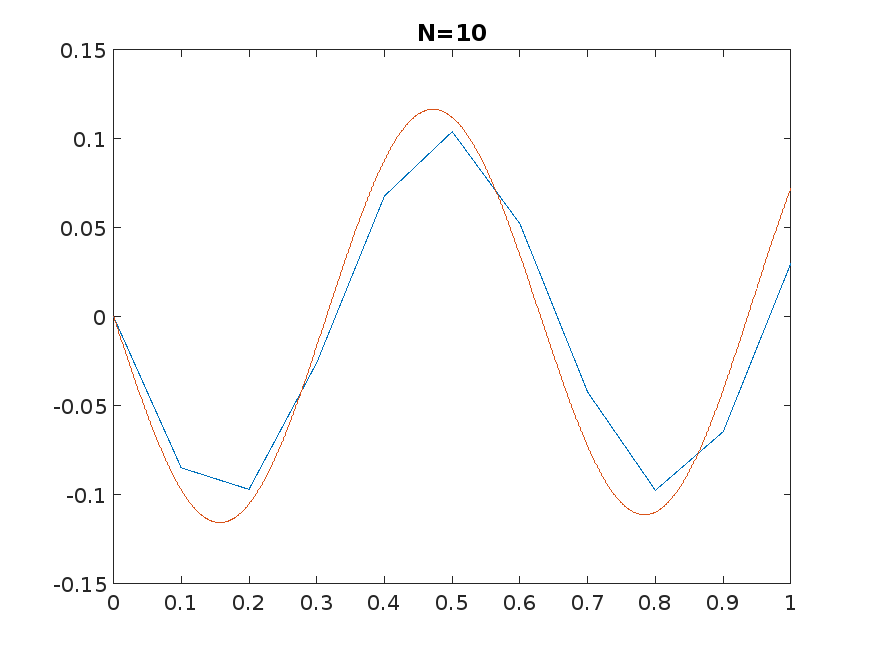
\includegraphics[width=0.3\textwidth]{./q1aN=10.png}
  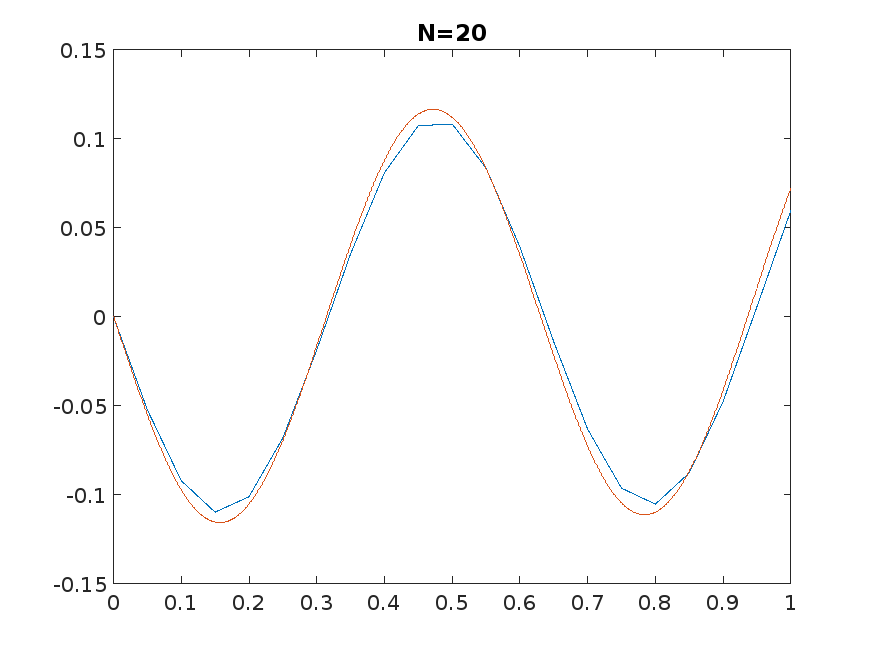
\includegraphics[width=0.3\textwidth]{./q1aN=20.png}
  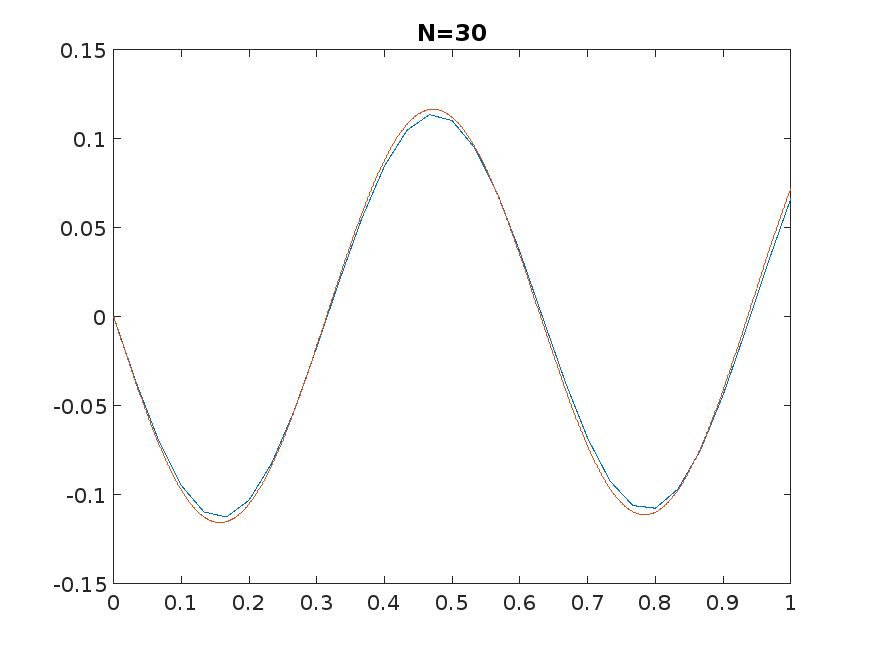
\includegraphics[width=0.3\textwidth]{./q1aN=30.png}
  \caption{Graphs for question 1e. Orange is exact and blue is numerical.}
  \label{fig:q1e}
\end{figure}

{\medskip\noindent\bf Question 1f.} All of the work for the previous parts have been to reduce the problem to one in the given form. Here $f=\alpha=\beta=0$ so $b=0$, and thus $Ku=-k^2Mu$. Letting $x=u, A=K,B=-M$ and $\lambda=k^2$, we see that this is the desired eigenvalue problem.

For finite differences, we discretize the equation $u''=-\lambda u$ to get $u_{n+1}-2u_n+u_{n-1}=-\lambda h^2 u_n$. The two boundary conditions give us that $u_{2}-2u_1=\lambda u_1$ and $u_{N}-u_{N-1}=h(0)=0$. Putting this in matrix form, we have
\[
  Au=\frac{1}{h^2}\begin{pmatrix} 2&-1&\cdots\\ -1&2&-1&\cdots\\ \vdots \\ &&\cdots&-1&2&-1\\ &&&\cdots &-1&1 \end{pmatrix}u=\lambda u
.\]

The eigenvalues (technically $\sqrt{\lambda}$ to keep it consistent with the later plot of $k_j$) for both methods can be seen in table \ref{tab:q1f}. 

\begin{table}[h]
\centering
\begin{tabular}{|c|c|}
\hline
\textbf{$k_{FE}=\sqrt{\lambda}$} & \textbf{$k_{DE}=\sqrt{\lambda}$} \\
\hline
1.5724 & 1.4946 \\
4.7561 & 4.4504 \\
8.0571 & 7.3068 \\
11.5542 & 10.0000 \\
15.3203 & 12.4698 \\
19.4002 & 14.6610 \\
23.7547 & 16.5248 \\
28.1465 & 18.0194 \\
31.9858 & 19.1115 \\
34.3236 & 19.7766 \\
\hline
\end{tabular}
\caption{Values of $k$ for finite element and difference equation.}
\label{tab:q1f}
\end{table}

The approximate expression for the eigenvalues is a solved problem, see e.g. \href{https://en.wikipedia.org/wiki/Eigenvalues_and_eigenvectors_of_the_second_derivative#Dirichlet-Neumann_Case}{here} for a derivation (I don't have time to rewrite it here):
\[
\lambda_k=-\frac{4}{h^2}\sin^2\left( \frac{\pi(k-0.5)}{(2N+1)} \right) 
.\]

For the plots, see figure \ref{fig:q1f}.

\begin{figure}[htpb]
  \centering
  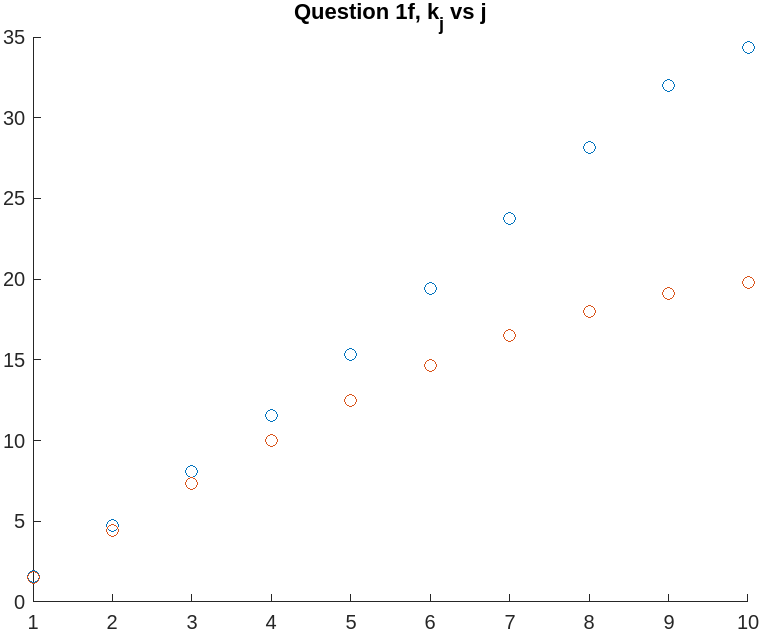
\includegraphics[width=0.4\textwidth]{./q1fkj.png}
  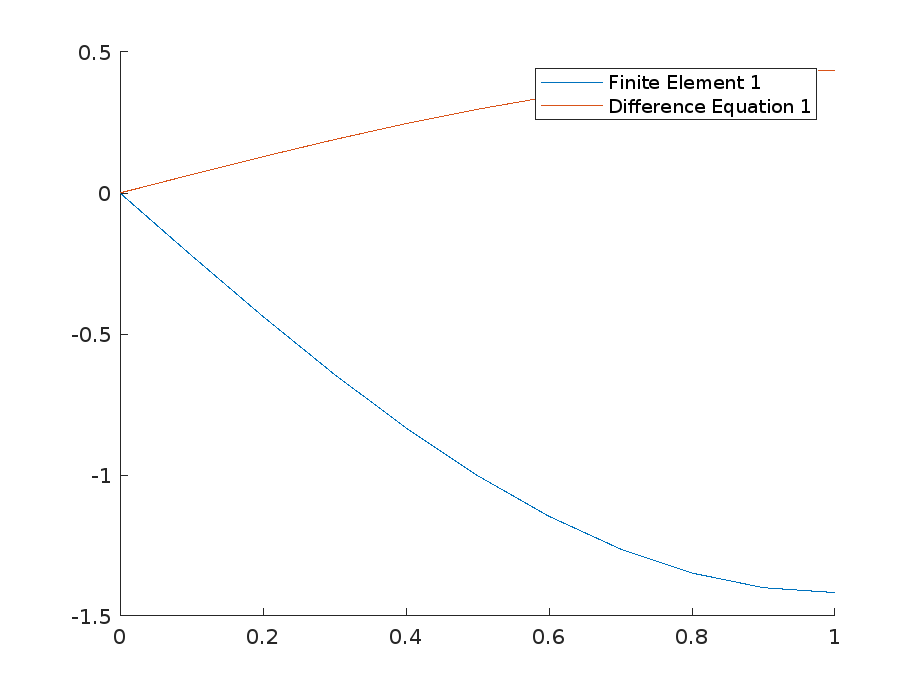
\includegraphics[width=0.4\textwidth]{./q1feig=1.png}
  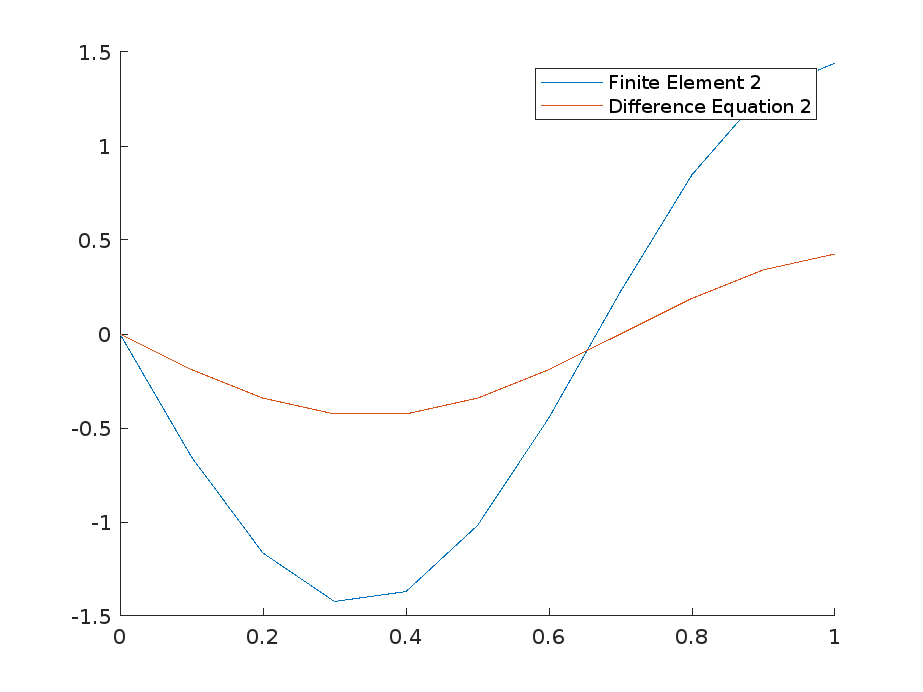
\includegraphics[width=0.4\textwidth]{./q1feig=2.png}
  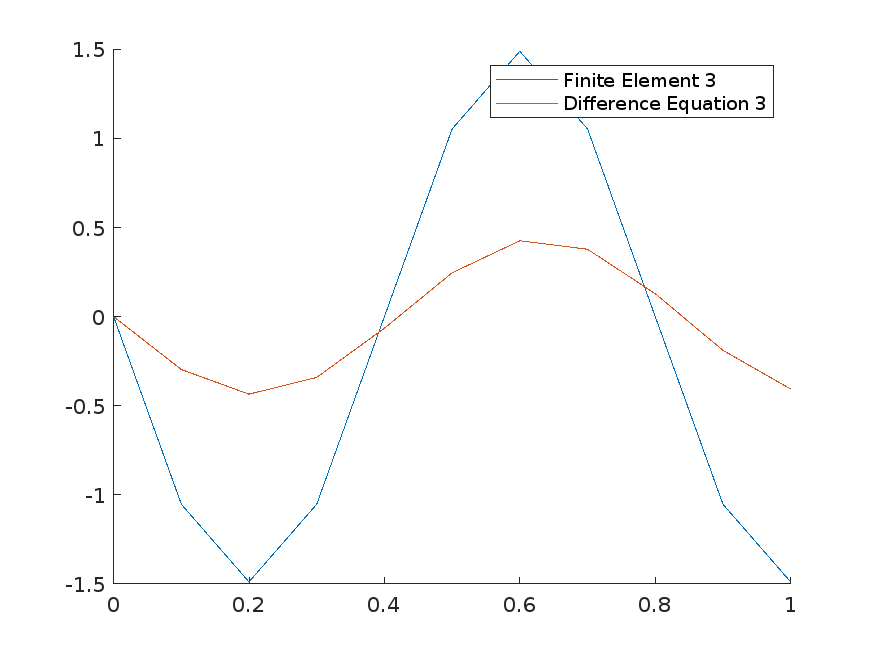
\includegraphics[width=0.4\textwidth]{./q1feig=3.png}
  \caption{Plots for question 1f. In $k_j$ plot, blue is finite element and orange is difference equation.}
  \label{fig:q1f}
\end{figure}

The code for this question is as follows:
\begin{lstlisting}
n = 10;
a = 0; b = 1;
h=(b-a)/n;
alpha = 0;
beta = 0;

K = full(gallery('tridiag',n,-1,2,-1));
K(n, n-1) = -1;
K(n, n) = 1;
K = (1/h) * K;

M = full(gallery('tridiag',n,1,4,1));
M(n, n) = 2;
M = (h/6) * M;

[V,D] = eig(K,M);
lambdaFE = diag(D);
eigenvecFE = V;

A = full(gallery('tridiag',n,-1,2,-1));
A(n,n) = 1;
A = A/(h^2);

[V,D] = eig(A);
lambdaDE = diag(D);
eigenvecDE = V;

figure;
scatter(1:n, lambdaFE.^0.5);
hold on;
scatter(1:n, lambdaDE.^0.5);
hold off;
title('Question 1f, k_j vs j')

x = linspace(a, b, n+1);
for i=1:3
    figure;
    hold on;
    plot(x, [0;eigenvecFE(:,i)], 'DisplayName', "Finite Element " + i);
    plot(x, [0;eigenvecDE(:,i)], 'DisplayName', "Difference Equation " + i);
    hold off;
    legend();
end


\end{lstlisting}

{\medskip\noindent\bf Question 2a.} From the main boundary value problem, we have that $\frac{D}{r}(rp_r)_r=0$, which has solutions in the form $p(r)=A+B\log r$. The boundary conditions forces $\lim_{r\to 0}r \frac{\partial p}{\partial r}=B=-\frac{Q_0}{2\pi D}$, and $p(R(t),t)=0\implies A=\frac{Q_0}{2\pi D}\log R(t)$. Putting this together we have $p(r,t)=\frac{Q_0}{2\pi D}\log \frac{R(t)}{r}$.

Using the Stefan condition for front velocity:
\[
\dot R(t)= -\frac{w_0^2}{\mu'}\frac{dp}{dr}\bigg]_{r=R(t)}=\frac{w_0^2}{\mu'}\frac{Q_0}{2\pi DR(t)}
.\]
Finally using separation of variables we can solve this differential equation:
\[
\int R(t)dR(t)=\int_0^{t}\frac{w_0^2}{\mu'}\frac{Q_0}{2\pi D}dt\implies R(t)=\sqrt{\frac{w_0^2Q_0t}{\mu'\pi D}}
.\]

{\medskip\noindent\bf Question 2bi.} Expanding, the equation to solve is $Lp=p_{rr}+\frac{1}{r}p_r=g(r,t)$. We can find the adjoint operator:
\[
\int_0^{R(t)}Gfrdr=\int_0^{R(t)}G\cdot (Lu)\cdot rdr=\int_0^{R(t)}G\left( ru''+u' \right) dr
.\]
From this point the self adjoint operator and associated boundary terms were derived in class (lecture 14), they are:
\[
  =\left[Ga_0u'+Ga_1u-(a_0G)'u\right]_{0}^{R(t)}+\int_{0}^{R(t)}u\left( (a_0G)''-(a_1G)'+a_2G \right) dr
\]
\[
  =\left[ru'G-rG'u\right]_0^{R(t)}+\int_0^{R(t)}u\left( rG''+G' \right) dr
.\]
Thus under the radial integration $L$ acts as self adjoint (there's probably some deeper reason for the way the algebra works out with the extra $r$, but from the algebra it works out at least). Thus to eliminate unknowns we want to find $G(s,r)$ such that $sG_{ss}(s,r)+G_s(s,r)=\delta(s-r)$ with $G(R(t),r)=0$ and $G(0,r)<\infty$. We already determined that the solution to the homogeneous equation is $p(r)=A+B\log r$. Thus we can split the Green's function into two parts:
\[
G(s,r)=\begin{cases}
  A_-+B_-\log s&0<s<r\\
  A_++B_+\log s&r<s<R(t)
\end{cases}
.\]
The boundary conditions force $B_-= 0$ and $A_+=-B_+\log R(t)$. Continuity forces that $A_-=B_+\log \frac{r}{R(t)}$. Thus we can write $G$ once again as
\[
G(s,r)=\begin{cases}
  B_+\log \frac{r}{R(t)}&0<s<r\\
  B_+\log \frac{s}{R(t)}&r<s<R(t)
\end{cases}
\]
\[
G_s(s,r)=\begin{cases}
  0&0<s<r\\
  \frac{B_+}{s}&r<s<R(t)
\end{cases}
.\]
The only condition left is the jump condition:
\[
\int_{r-\epsilon}^{r+\epsilon}sG_{ss}+G_sds=\int_{r-\epsilon}^{r+\epsilon}(sG_s)_sds=sG_s\bigg|_{r-\epsilon}^{r+\epsilon}=r\left( G_s(r_+,r)-G_s(r_-,r) \right)=\int_{r-\epsilon}^{r+\epsilon}s\delta(r-s)ds=r
\]
\[
\implies 1=(B_+-0)\implies B_+=1
.\]
We can then get a final formulation for $G$:
\[
G(s,r)=\begin{cases}
  \log \frac{r}{R(t)}&0<s<r\\
  \log \frac{s}{R(t)}&r<s<R(t)
\end{cases}.\]
The only boundary term is $\lim_{s\to 0}su'(s)G(s,r)=-\frac{Q_0}{2\pi D}\log \frac{r}{R(t)}$. Putting this together we can determine an expression for $p(r,t)$ in terms of $R(t)$ and $g(r,t)$:
\[
p(r,t)=-\frac{Q_0}{2\pi D}\log \frac{r}{R(t)}+\int_0^{r}\log \frac{r}{R(t)}g(s)sds+\int_r^{R(t)}\log \frac{s}{R(t)}g(s)sds
.\]
Finally, using the explicit expression for $f(r,t)$ given in the question we get
\[
p(r,t)=-\frac{Q_0}{2\pi D}\log \frac{r}{R(t)}+\int_0^{r}\log \frac{r}{R(t)}\frac{C'H(t-t_0(s))}{D\sqrt{t-t_0(s)}}sds+\int_r^{R(t)}\log \frac{s}{R(t)}\frac{C'H(t-t_0(s))}{D\sqrt{t-t_0(s)}}sds
.\]

{\medskip\noindent\bf Question 2bii.} Plugging in $r=R(t)$:
\[
  p_r(r,t)=-\frac{Q_0}{2\pi Dr}+\left( \frac{1}{r} \right) \int_{0}^{r}g(s)sds+rg(r)\log \frac{r}{R(t)}-rg(r)\log \frac{r}{R(t)}
\]
\[
  p_r(r,t)=-\frac{Q_0}{2\pi Dr}+ \int_{0}^{r}g(s)\frac{s}{r}ds
\]
\[
  p_r(R(t),t)=-\frac{Q_0}{2\pi DR(t)}+ \int_{0}^{R(t)}g(s)\frac{s}{R(t)}ds
.\]
Plugging this in to the Stefan condition:
\[
\dot R(t)=-\frac{w_0^2}{\mu'}\frac{dp}{dr}\bigg|_{r=R}=-\frac{w_0^2Q_0}{2\mu'\pi DR(t)}+ \frac{w_0^2}{\mu'R(t)}\int_{0}^{R(t)}\frac{C'H(t-t_0(s))}{D\sqrt{t-t_0(s)}}sds
.\]
Make the suggested change of variables $s=R(\tau),ds=\dot R(\tau) d\tau$. Then $\tau=R^{-1}(s)=t_0(s)$, $s=0\implies \tau =0$ and $s=R(t)\implies \tau=t$. Then we get
\[
\dot R(t)R(t)=\phi(R,\dot R)=-\frac{Q_0}{2\pi w_0}+\frac{1}{w_0}\int_0^{t}\frac{C' H(t-\tau)\dot R(\tau)R(\tau)}{\sqrt{t-\tau}}d\tau
.\]
Note that $\tau<t$ throughout the whole integral, so the Heavyside function is always 1. Then we have:
\[
\phi(R,\dot R)=-\frac{Q_0}{2 \pi w_0}+\frac{C'}{w_0}\int_0^{t} \frac{\phi(R,\dot R)}{\sqrt{t-\tau}}d\tau
.\]

{\medskip\noindent\bf Question 2biii.} Since the integral given is in the form of a convolution integral, the Laplace transform of the whole thing will be the product of the Laplace transforms of each one. Let $F(s)=\mathcal L \{\phi(R,\dot R)\}$. Then we have
\[
\mathcal L \{\phi(R,\dot R)\}=F(s)=\mathcal L \left\{-\frac{Q_0}{2 \pi w_0}+\frac{C'}{w_0}\int_0^{\infty} \phi(R,\dot R)\frac{H(t-\tau)}{\sqrt{t-\tau}}d\tau\right\}= F(s)=-\frac{Q_0}{2\pi w_0 s}+\frac{C'}{w_0}F(s) \sqrt{\frac{\pi}{s}}
\]
\[
  \implies F(s)=- \frac{Q_0}{2\pi w_0s}\left( 1-\frac{C'}{w_0}\sqrt{\frac{\pi}{s}} \right)^{-1}=-\frac{Q_0\sqrt{s}}{2\pi s(w_0\sqrt{s}-C'\sqrt{\pi})}= \frac{Q_0}{2\pi^{3 /2} C'}\frac{1}{s-w_0 \sqrt{s} /(C'\sqrt{ \pi})}
.\]

{\medskip\noindent\bf Question 2biv.} We can invert the Laplace transform using the given transform. Let $\alpha=-\frac{w_0}{C'\sqrt{\pi}}$ and $A=\frac{Q_0}{2\pi^{3 /2}C'}$ (I'd give it 50/50 odds I've dropped a constant by this point), and compute:
\[
  \phi(R,\dot R)=\mathcal L^{-1}\{F(s)\}=Ae^{\alpha^2 t}\text{erfc}\left( \alpha \sqrt{t} \right)
.\]
We can then use separation of variables to solve for $R$:
\[
\int RdR=\frac{1}{2}R^2=\int_0^{t} \phi(R,\dot R)dt=\frac{A}{\alpha^2}\left( e^{\alpha^2t}\text{erfc}\left( \alpha t ^{1 /2} \right) -1 \right) +\frac{2At ^{1 /2}}{\alpha \pi^{1 /2}}
\]
\[
  \implies R(t)=\sqrt{\frac{2A}{\alpha^2}\left( e^{\alpha^2t}\text{erfc}\left( \alpha t ^{1 /2} \right) -1 \right) +\frac{4At ^{1 /2}}{\alpha \pi^{1 /2}}}
.\]
The question asks to find $\dot R$ in the process of finding $R$, but given I didn't need to and the expression for $R$ seems lengthy to differentiate I assume it's not necessary. Our expression for $p(r,t)$ is the same except now $R(t)$ is known using the above equation:
\[
p(r,t)=-\frac{Q_0}{2\pi D}\log \frac{r}{R(t)}+\int_0^{r}\log \frac{r}{R(t)}\frac{C'}{D\sqrt{t-t_0(s)}}sds+\int_r^{R(t)}\log \frac{s}{R(t)}\frac{C'}{D\sqrt{t-t_0(s)}}sds
.\]

{\medskip\noindent\bf Question 2bva.} Given $F(R)=\frac{1}{2}R^2$ in my case this seems too simple and I may have made a mistake at this point, but I can't seem to find it and I'll continue nonetheless. See the radius in figure \ref{fig:q2va}. The code used was:
\begin{lstlisting}
Q=1;C=1;mu=1;w0=1;

alpha = -w0/C/pi^(0.5);
A = Q/(2*pi^(3/2)*C);

tmax = 500;
t = linspace(0,tmax,1000);

R = (2*A/alpha^2*(exp(alpha^2.*t).*erfc(alpha*t.^(1/2))-1)+4*A*t.^(1/2)/alpha/pi^(1/2)).^(0.5);

plot(t, R);
title("Radius over time")
\end{lstlisting}

\begin{figure}[htpb]
  \centering
  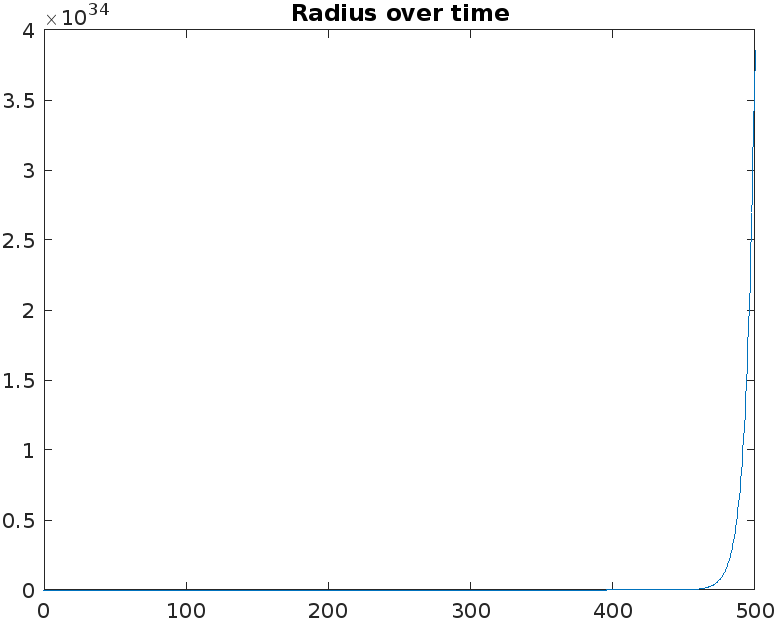
\includegraphics[width=0.8\textwidth]{q2va}
  \caption{Graph for question 2bva. It grows exponentially which doesn't seem reasonable given the version of the ODE without the sink didn't, but I don't have time to figure out what's wrong.}
  \label{fig:q2va}
\end{figure}

{\medskip\noindent\bf Question 2bvb.} Ran out of time, sorry.

{\medskip\noindent\bf Question 3a.} Let $v$ be an arbitrary perturbation, then we can integrate by parts:
\[
\int_0^{R(t)}v \frac{1}{r}\left( rp_r \right)_r rdr=v(rp_r)\bigg|_0^{R(t)}-\int_0^{R(t)}v'p'rdr=0
.\]
% We know $\lim_{r\to 0}rp_r$ but not $p_r(R(t))$, so we need $v(R(t))=0$ and $v(0)<\infty$. Thus we're looking for $u$ such 
Thus the weak form is to find $u$ such that the above equation is satisfied for all $v\in H_0^{1}$.

{\medskip\noindent\bf Question 3b.} Let $p(r)=\sum_{n=0}^{N}p_n N_n(r)=\sum_{n=0}^{N-1}p_n N_n(r)$ and $v(r)=\sum_{n=0}^{N-1}v_n N_n(r)$. Plugging this into the equation:
\[
\int_0^{R(t)}\left( \sum_{n=0}^{N-1}p_nN_n' \right) \left( \sum_{m=0}^{N-1}v_mN_m' \right) rdr=v_0 \frac{Q_0}{2\pi D}
\]
\[
  \implies \sum_{m=0}^{N-1}v_m\left( \sum_{n=0}^{N-1}u_n\left( \int_0^{R(t)}N_n'N_m'r dr \right)  \right)=v_0 \frac{Q_0}{2 \pi D} \implies Ku=b
,\]
where $b_0=\frac{Q_0}{2\pi D}$ and $b_i=0\forall i>0$, and $K$ is the stiffness matrix. To construct $K$, consider an individual element $e$. Then similar to question 1 by parameterizing by $\xi$ and using linear basis functions $N_a(\xi),N_b(\xi)$, we get
\[
r(\xi)=r_{e-1}N_1(\xi)+r_e N_2(\xi)= \frac{x_e+x_{e-1}}{2}+\frac{h\xi}{2}
.\]
\[
\implies \int_{x_{e-1}}^{x_e} N_m'N_n'rdr=\int_{-1}^{1}\frac{dN_a}{d\xi}\frac{d\xi}{dr}\frac{dN_b}{d\xi}\frac{d\xi}{dr}\frac{dr}{d\xi}\left( \frac{x_e+x_{e-1}}{2}+\frac{h\xi}{2} \right)  d\xi
\]
\[
=\frac{2}{h}\int_{-1}^{1}\frac{\xi_a\xi_b}{4}\left( \frac{x_e+x_{e-1}}{2}+\frac{h\xi}{2} \right)d\xi= \frac{2}{h}\int_{-1}^{1}\frac{\xi_a\xi_b\left( x_e+x_{e-1} \right) }{8}d\xi
\]
\[
  \implies K_{ab}^{e}=\frac{x_e+x_{e-1}}{2h}\begin{pmatrix} 1&-1\\-1&1 \end{pmatrix} 
.\]
The final matrix $K$ can be constructed by adding these individual element matrices together. Unlike the Hemoltz case this doesn't sum in a clean way since each of these components has radial dependence that makes it tricky to write explicitly.

{\medskip\noindent\bf Question 3c.} See figure \ref{fig:q3c} for the plot of the finite element and exact solution. As can be seen, they are extremely close and the finite element provides a good approximation of the real value. The code used was:

\begin{figure}[htpb]
  \centering
  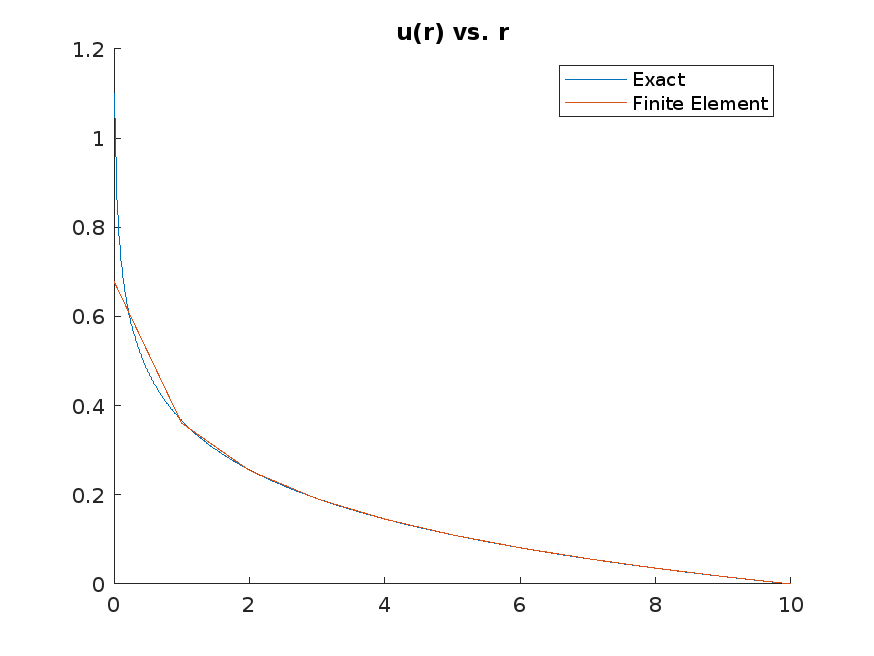
\includegraphics[width=0.8\textwidth]{q3c}
  \caption{Finite element and exact solution for question 3c.}
  \label{fig:q3c}
\end{figure}

\begin{lstlisting}
n = 10;
a=0; b=10;
h = (b-a)/n;
Q=1;D=1;

exact = @(x) Q./(2*pi*D)*log(b./x);

x = linspace(a,b,n+1);
xe = linspace(a,b,1000);
K = zeros(n);
for i=2:n
    tmp = (x(i-1)+x(i))/2/h;
    K(i,i) = K(i,i) + tmp;
    K(i-1,i-1) = K(i-1,i-1) + tmp;
    K(i,i-1) = K(i,i-1) - tmp;
    K(i-1,i) = K(i-1,i) - tmp;
end

K(n,n) = K(n,n) + (x(n)+x(n+1))/2/h;

b = zeros(1,n);
b(1)=Q/(2*pi*D);

p = [b / K, 0];

figure;
hold on;
plot(xe, exact(xe), 'DisplayName', "Exact")
plot(x, p, 'DisplayName', "Finite Element")
hold off;
title("u(r) vs. r")
legend;

\end{lstlisting}

{\medskip\noindent\bf Question 3d+e.} Ran out of time.

\end{document}
